\documentclass[conference]{IEEEtran}
%	\IEEEoverridecommandlockouts
\usepackage{cite}
\usepackage{amsmath,amssymb,amsfonts}
%	\usepackage{algorithmic}
\usepackage[dvipdfmx]{graphicx}
\usepackage{graphicx}
\usepackage{color}
\usepackage{textcomp}
\usepackage{xcolor}
\definecolor{blue}{rgb}{0.00, 0.00, 1.00}
\usepackage{listings}
\usepackage{datetime2}
\usepackage{algorithm}
\usepackage{algorithmicx}
\usepackage{algpseudocode}
%	\usepackage{comment}
\def\BibTeX{{\rm B\kern-.05em{\sc i\kern-.025em b}\kern-.08em T\kern-.1667em\lower.7ex\hbox{E}\kern-.125emX}}
\lstset{
  language={Fortran},
  basicstyle={\ttfamily},
  identifierstyle={\small},
  %	commentstyle={\smallitshape},
  % keywordstyle={\small\bfseries},
  keywordstyle={\small},
  ndkeywordstyle={\small},
  %	stringstyle={\small\ttfamily},
  frame={tb},
  breaklines=true,
  columns=[l]{fullflexible},
  numbers=left,
  xrightmargin=0zw,
  xleftmargin=2zw,
  numberstyle={\scriptsize},
  stepnumber=1,
  numbersep=1zw,
  lineskip=-0.5ex,
  %	belowcaptionskip=10pt,abovecaptionskip=10pt
}


\begin{document}

\title{
%
%	\textcolor{blue}{as of \DTMnow} \\
%
Performance evaluation and visualization of scientific applications using PMlib
}

\author{
\IEEEauthorblockN{1\textsuperscript{st} Kazunori Mikami}
\IEEEauthorblockA{\textit{Flagship 2020 Project} \\
\textit{Riken R-CCS}\\
Kobe, Japan \\
kazunori.mikami@riken.jp}
\and
\IEEEauthorblockN{2\textsuperscript{nd} Kenji Ono}
\IEEEauthorblockA{\textit{RIIT, Kyushu University} \\
\textit{Riken R-CCS}\\
Fukuoka, Japan \\
keno@\{cc.kyushu-u.ac, riken\}.jp}
\and
\IEEEauthorblockN{3\textsuperscript{rd} Jorji Nonaka}
\IEEEauthorblockA{\textit{HUD unit} \\
\textit{Riken R-CCS}\\
Kobe, Japan \\
jorji@riken.jp}
}

\maketitle

\begin{abstract}
Computational performance of scientific applications on HPC systems
is often much lower than user expectation based on the system's maximum
performance.
To correctly understand this performance gap, multi-perspective evaluation
becomes important.
For instance, from system architecture perspective,
evaluating the characteristics of micro architecture elements such as
processor core and memory is valueable.
And from user perspective, correlating the theoretical computation coded
as a source program with the actual computation workload produced by compilers
is valueable.
An open source library called PMlib was developed to address such synthetic
evaluation.
PMlib provides the way to report the arithmetic/application workload
counted manually from a source code,
as well as the actually executed system workload.
It also provides the detail utilization report of processor specific hardware
including the categorized SIMD instruction statistics, the layered cache
hit/miss rate, and the corresponding bandwidth up to memory,
which are captured via hardware performance counters (HWPC).
Using PMlib, users can conduct synthetic analysis of application
performance, and obtain hints for further optimized execution of applications.
\end{abstract}

\begin{IEEEkeywords}
performance evaluation,
arithmetic workload,
HWPC workload,
performance visualization,
open source library,
PMlib
\end{IEEEkeywords}

\section{Introduction}
In the development and productive phase of scientific applications,
the performance evaluation is frequently conducted on target HPC systems.
in order to understand the performance characteristics
of the application on the target system, and to explore the possibility of
applying further optimization to the application for the reduction of elapsed time.
Therefore,
depending on the type of scientific applications and HPC systems,
it is frequently observed that
the sustained computational performance of applications
systems is much lower than the theoretical maximum performance
expected from the system specification.

Prededing studies to account for this gap between the achieved
performance and the maximum performance have been addressed mostly from
architecture point of view, e.g., 
utilization of parallel functional units,
and locality of data residing on memory/cache hierarchy.

Generally, the performance of applications is measured in the unit of conducted workload/elapsed time.
It should be reminded that there are two categories to define the workload
of a program for the performance measurement. 
One is the arithmetic workload defined in the applications source program,
and the other is the system workload actually executed on HPC systems
that is represented as machine instructions  and is measured with
hardware performance counters (HWPC).
The difference in the performance based on these two workload definitions
can be significant as explained in section \ref{workload-evaluation},
and is sometimes confusing to application users for understanding
its behaviour.

PMlib~\cite{PMlib:webpage-public}, an open source library for performance
evaluation, has the functionality
to explicitly measure the arithmetic workload counted in the source program
using manually formulated argument, as well as the functionality
to automatically measure the HWPC event base workload,
thus providing users an option to compare the difference in workloads.

In measuring the HWPC events, PMlib utilizes PAPI~\cite{PAPI:5.6} low level API.
PMlib has its own scheme to choose the related HWPC event sets and to sort out
the event statistics according to run-time environment variables, making it
easier to extract the statistics of interest.
Choosing the correct set of events for specific processor type and
translating the accumulated counts into meaningful performance index can be
non-trivial work if without PMlib.
The output information from PMlib is a blocked text report based on
the time averaged performance statistics by default.
It also produces the
Open Trace Format~\cite{Knupfer:2006},~\cite{OTF:webpage-public}
tracing file reflecting
the shorter interval statistics which can be read by a Web browser
visualization tool.  % TRAiL~\cite{trail}~.%

In this paper, the difference between the arithmetic workload and the system
workload is clarified.
Next, the PMlib's useful feature for the performance evaluation is shown.
Finally, some examples of the performance evaluation using PMlib
are shown indicating the merit obtained from multi-perspective analysis.

%%
\section{Computational workload and Performance evaluation}
\label{workload-evaluation}

%
\subsection{User perspective}
\label{subsection:user-perspective}

The term "computational workload" for scientific application developpers
is generally perceived as the total volume of arithmetic operations,
expressed by the formulas in the source code written in Fortran/C/C++.

The workload at this level can be simply represented as below:
%	\begin{align}
%	\end{align}
\begin{equation}\label{eq:arithmetic-workload}
	Workload = \sum_{i=1}^{types} W_{ops}(i)
\end{equation}
where $ W_{ops}(i) $ is the number of operations for the
corresponding arithmetic type such as
1:add, 2:sub, 3:mult, 4:div, 5:max, 6:min, 7:sqrt, etc.

In the development phase of the HPC applications, practical developers
choose and deploy the numerical algorithm which requires the least
amount of arithmetic operations through the scientific consideration,
aiming to reduce the elapsed time to obtain the desired simulation results.
The workload in this context is named arithmetic workload in this paper.

The formulas in the source code are then compiled to corresponding assembly
instructions.
Each arithmetic statement is mapped to a sequence of multiple instructions.
``Weight factor'' is used to map the original arithmetic operations to the
generated instructions to quantify the relationship.
Assuming a simple weight factor $ c $ for each type of
arithmetic operations, 
the revised workload can be represented as follows:
\begin{equation}\label{eq:application-workload}
		Workload = \sum_{i=1}^{types} \left(c(i)\times W_{ops}(i)\right)
\end{equation}
% workload_{system}

\noindent This workload formula is named ``application workload'' in this paper.
Equation~(\ref{eq:application-workload})
is a simple representation of the workload observed in application level 
using the original arithmetic,
and provides easy-to-understand relationship between the change
in the algorithm and the resulting change in the application workload.

The application performance is evaluated based on the elapsed time as below.
\begin{align}\label{eq:performance-workload-time}
Performance = Workload / Time 
\end{align}

\noindent For example, Linpack (HPCC)~\cite{}
workload is calculated based on the arithmetic workload formula
using the addition and multiplication terms.
\begin{align}
		Workload & = W_{ops}(add) + W_{ops}(mult) \\
		W_{ops}(add) & = W_{ops}(mult) = 1/3 N^{3} + 3/4 N^{2}
\end{align}
where N is the size of the matrix to be solved.
Linpack performance value "flops" is reported using this workload as
\begin{align*}
Gflops = N^{2} \times ( 2/3 * N + 3/2 ) \times 1.0^{-9} / Time 
\end{align*}
In Linpack example, the application performance is based on
the same weight factor $ c = 1.0 $ 
for both addition and multiplication, which is actually reflecting the
arithmetic workload and performance.

The workload formulation in the form of
\eqref{eq:arithmetic-workload}
or
\eqref{eq:application-workload}
provides the general idea of the theoretical workload requirement by the
application.
PMlib can be used to formulate these arithmetic and application workload
as explained in section~\ref{section:PMlib}.

%
\subsection{System perspective}
\label{subsection:system-perspective}

It may be difficult to formulate the arithmetic workload
or the application workload for large-scale applications.
Even if the workload formulation is accomplished,
the mapping of weight factor may become complicated.

Mapping mathematical functions to the native instructions
depends not only on the systems architecture but also on the compilers
and its optimization options.
There are multiple choices of available instructions for the same
arithmetic operation on modern processors.
The choice of instructions from scalar/vector syntax is made by the
compiler optimization strategy.
For instance,
in vector operation, the degree of parallelism, i.e. width of simultaneous data
operation, with the effect of loop length is influential.
In scalar operation, the data locality is influential.
Run-time hardware behavior including out-of-order execution can not
be reflected to a static weight factor.
A simple instruction latency and throughput model may not taking into account.

Now the workload and performance are focused on from the system perspective.
The micro architecture elements including the number of computation cores
in a processor, the degree of parallelism inside each core,
the depth of cache/memory hierarchy and the data move rate at each hierarchy,
all have relational impact to how the machine instructions are executed,
thus leading to sustained computing performance.
The fact that the actual numerical computation is accomplished by the
limited set of hardware components, and that the HWPC is available
on modern HPC systems, makes it more practical to obtain the HWPC statistics
and to analyze them for performance evaluation.
Through appropriate APIs, HWPC statistics can be accessed, so does PMlib.

PMlib utilize PAPI low-level APIs to accomplish this,
and calculates the computing workload from the executed instructions.
It provides the processor specific hardware utilization report
including categorized SIMD instruction statistics,
layered cache hit/miss rate, and the corresponding bandwidth up to memory.
It utilizes PAPI low level API for obtaining HWPC event statistics.
PAPI has its own HWPC event mnemonics for each type of proccessors.
For example, floating point operations on
Intel Xeon Skylake Gold processor % no citation \cite{skylake-1} 
are measured as the following events.
\vspace{1mm}
%	\begin{lstlisting}[caption={Intel Xeon Skylake f.p. SIMD operations}]
%	\end{lstlisting}
\begin{quote}
\begin{small}
\begin{verbatim}
fpsp1  : "FP_ARITH:SCALAR_SINGLE";
fpsp4  : "FP_ARITH:128B_PACKED_SINGLE";
fpsp8  : "FP_ARITH:256B_PACKED_SINGLE";
fpsp16 : "FP_ARITH:512B_PACKED_SINGLE";
fpdp1  : "FP_ARITH:SCALAR_DOUBLE";
fpdp2  : "FP_ARITH:128B_PACKED_DOUBLE";
fpdp4  : "FP_ARITH:256B_PACKED_DOUBLE";
fpdp8  : "FP_ARITH:512B_PACKED_DOUBLE";
\end{verbatim}
\end{small}
\end{quote}
\vspace{1mm}
The sum of these operations multiplied by the corresponding width
of the SIMD instruction gives the floating point operation workload
including single and double precision data types.
%	\begin{multline}
%	W_{hwpc} = fpsp1 + fpdp1 \\
%		+ 4.0*fpsp4 + 8.0*fpsp8 + 16.0*fpsp16 \\
%		+ 2.0*fpdp2 + 4.0*fpdp4 + 8.0*fpdp8;
%	\end{multline}
\begin{align}
	\mathrm{W}_{hwpc} & = \mathrm{fpsp1} + \mathrm{fpdp1} \nonumber \\
			& + 4.0*\mathrm{fpsp4} + 8.0*\mathrm{fpsp8} + 16.0*\mathrm{fpsp16} \nonumber \\
			& + 2.0*\mathrm{fpdp2} + 4.0*\mathrm{fpdp4} + 8.0*\mathrm{fpdp8}
\end{align}

\noindent The workload measured in this fashion is named as HWPC workload,
and the evaluated performance as HWPC performance.
HWPC performance is commonly used in the HPC systems evaluation.

%
\subsection{Difference in workloads}
\label{subsection:difference-in-workloads}

In this section, an example is shown that exibits of the significant
difference between the user perspective arithmetic workload and
the system perspective workload.

Fig.~\ref{fig:workload-user} and Fig.~\ref{fig:workload-system} show
the performance baed on the workload defined in above context.
The vertical axis shows the performance corresponding to workload as
defined by \eqref{eq:performance-workload-time}.
In order to obtain these results, PMlib user mode report and PMlib HWPC mode
report were used.
% IVY case
Fig.~\ref{fig:workload-difference} shows the difference between
them as the ratio.
%
% FX100 case
% To be moved to section \ref{subsection:basic-kernels}.
%	The difference ranges from 1.0 to 18.0 depending on the type of
%	arithmetic, and stays mostly constant over various loop length.
%	The major reason for this parcular difference comes from the number of
%	instructions needed to
%	compute square root and division.
%
The execution elapsed time
of Fig.~\ref{fig:workload-user} and Fig.~\ref{fig:workload-system} are
almost identical, so the difference observed in
Fig.~\ref{fig:workload-difference} 
actually represents the difference of the workload.
The ratio ranges from 1.0 to 2.5 depending on the type of
arithmetic, and it varies depending on the loop length.

%	\begin{figure}[tb]
%	\centering
%	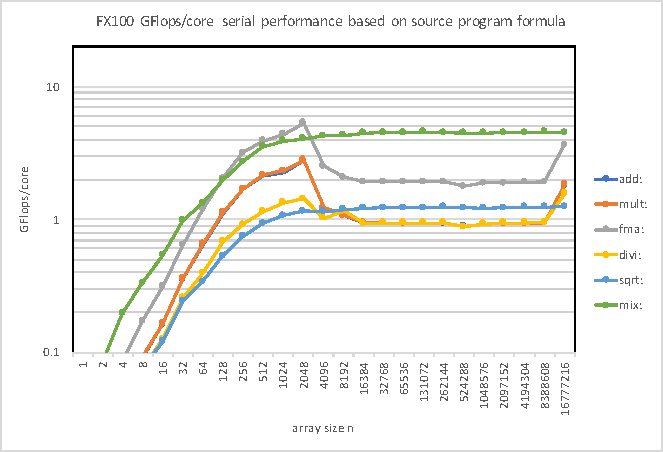
\includegraphics[width=0.45\textwidth]{figs/workload-user.pdf}
%	\caption{workload-user}
%	\label{fig:workload-user}
%	\end{figure}
\begin{figure}[tb]
%\begin{minipage}{0.49\hsize}
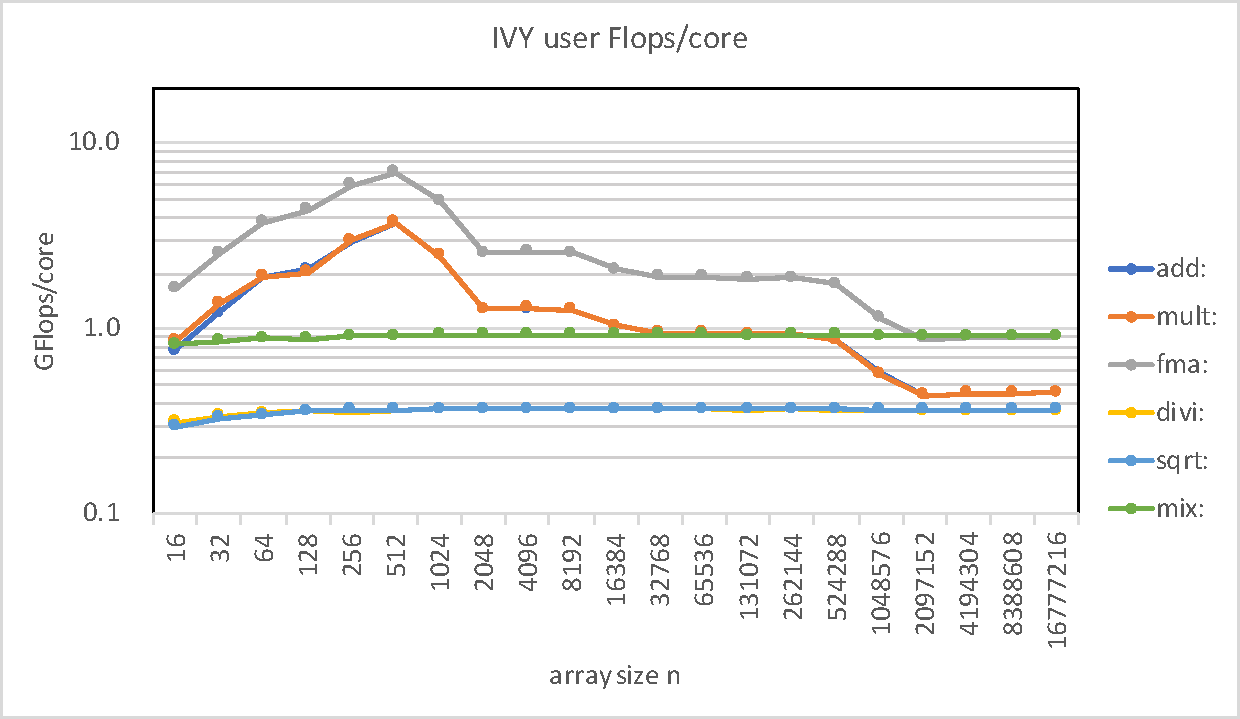
\includegraphics[width=0.5\textwidth]{figs/workload-ivy-user.pdf}
\caption{user perspective workload and performance}
\label{fig:workload-user}
\end{figure}
%\end{minipage}
\begin{figure}[tb]
%\begin{minipage}{0.49\hsize}
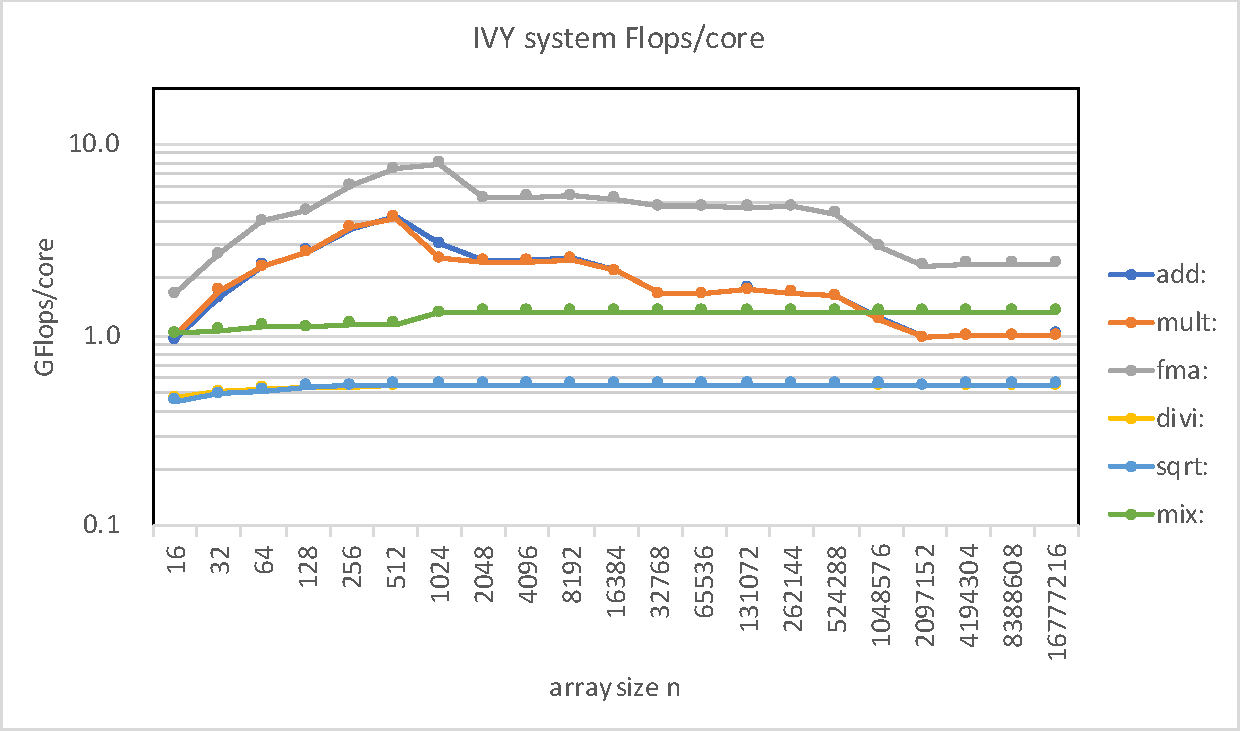
\includegraphics[width=0.5\textwidth]{figs/workload-ivy-system.pdf}
\caption{system perspective workload and performance}
\label{fig:workload-system}
%\end{minipage}
\end{figure}
%
\begin{figure}[tb]
%\begin{minipage}{0.49\hsize}
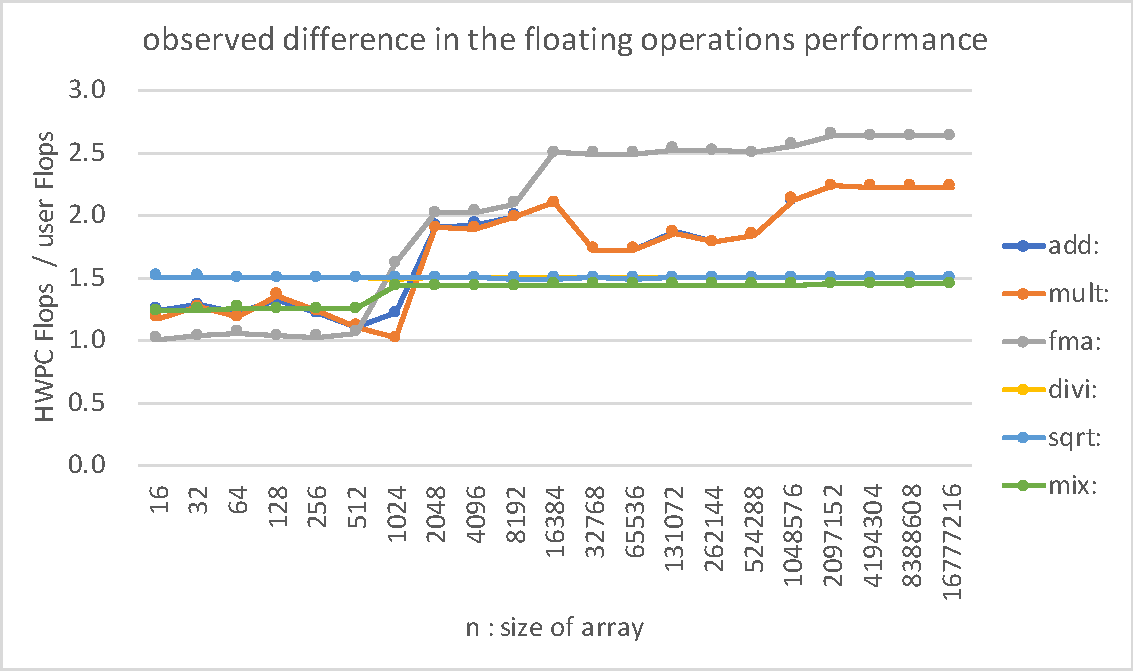
\includegraphics[width=0.5\textwidth]{figs/workload-ivy-difference.pdf}
\caption{difference of two workload}
\label{fig:workload-difference}
%\end{minipage}
\end{figure}

This simple example clearly indicates that the performance evaluation of
scientific applications on HPC systems must be associated with the clear
definition of workload, and that, if conditions allows, evaluation should be
conducted both in user perspective and in system perspective.
Detail analysis of a similar example is given in section
\ref{subsection:basic-kernels}.

%%
\section{Performance Monitoring Library}
\label{section:PMlib}

%
\subsection {Overview of PMlib}
PMlib is an open source library to monitor the scientific applications
performance and is able to measure the listed types of workload discussed
in the previous
section, i.e. arithmetic, application and HWPC workload.
Users can insert the start/stop API statements provided in the source code.
Each measuring section has minimal properties such as name, type of operation,
exclusiveness, and the workload value.
The report is output from PMlib is classified into threads, processes, sections,
depending on the controlling environment variable.

%
\subsection{PMlib API}
%\label{subsection:PMlib-API}
PMlib provides APIs for C++ and Fortran programs.
There are only handful APIs which must be called in most applications.
C++ APIs are shown in Table~\ref{tab:PMlib-API}. 
Equivalent Fortran APIs that follow similar naming convention as
$f\_pm\_${\footnotesize{C++API}} are also provided.

\begin{table}[htb]
\scriptsize
\caption{list of basic APIs provided by PMlib}
\label{tab:PMlib-API}
\footnotesize
\begin{tabular}{l|l|l} \hline
\scriptsize
C++	& function	&	arguments	\\ \hline \hline
initialize	& initial setup	& number of sections (optional)	\\ %\hline
setProperties	& set sections property	& label, type, exclusiveness \\ %\hline
start	& start of section	& label \\ %\hline
stop	& end of section	& label, arithmetic workload (optional)	\\ %\hline
print	& basic report	& filename, comments, sort order	\\ %\hline \hline
printDetail	& per process report	& filename, sort order	\\ %\hline
printThreads	& per thread report	& filename, sort order	\\ \hline
\end{tabular}
\end{table}

Following example shows a Fortran program calling PMlib.

%	\begin{lstlisting}[caption={using PMlib in Fortran program}]
\begin{lstlisting}
program main
call f_pm_initialize (Nsections)
call f_pm_setproperties ("section1",icalc,iexcl)
call f_pm_start ("section1")
call some_computation (fops)
call f_pm_stop ("section1",fops,ncall)
call f_pm_print ("",isort)
call f_pm_printdetail ("",ilegend,isort)
end
\end{lstlisting}

%
\subsection{Choosing workload type}
\label{subsection:Choosing-workload-type}

The choice of arithmetic workload or HWPC workload is made by a
run-time environment variable HWPC\_CHOOSER.
Possible choice of HWPC\_CHOOSER value is:
\begin{quote}
\begin{small}
%	\begin{verbatim}
FLOPS\textbar BANDWIDTH\textbar VECTOR\textbar CACHE\textbar CYCLE%
\textbar user
%	\end{verbatim}
\end{small}
\end{quote}

%If the arithmetic workload is measured,
PMlib API accepts the argument holding the value or the formula of the workload that contains the number of arithmetic inside the section sandwiched by start and stop statements.
The number of arithmetic operations or the formula must be explicitly
provided by users. Counting up the operation in source can be a tedious job.
If the application is written in Fortran program,
we can take advantage of the related research~\cite{Hoshimoto:2015},~\cite{ccaebt:HPCAsia2018}
to let the parser program analyze the arithmetic operations
included in Fortran source blocks and produce JSON intermediate report.
Then, a second filter can be used to produce the
Fortran source program including PMlib API calls with
provisioned argument for PMlib.
Fig.~\ref{fig:ccaebt4PMlib} shows the schematic flow to accomplish this process.

\begin{figure}[tb]
\centering
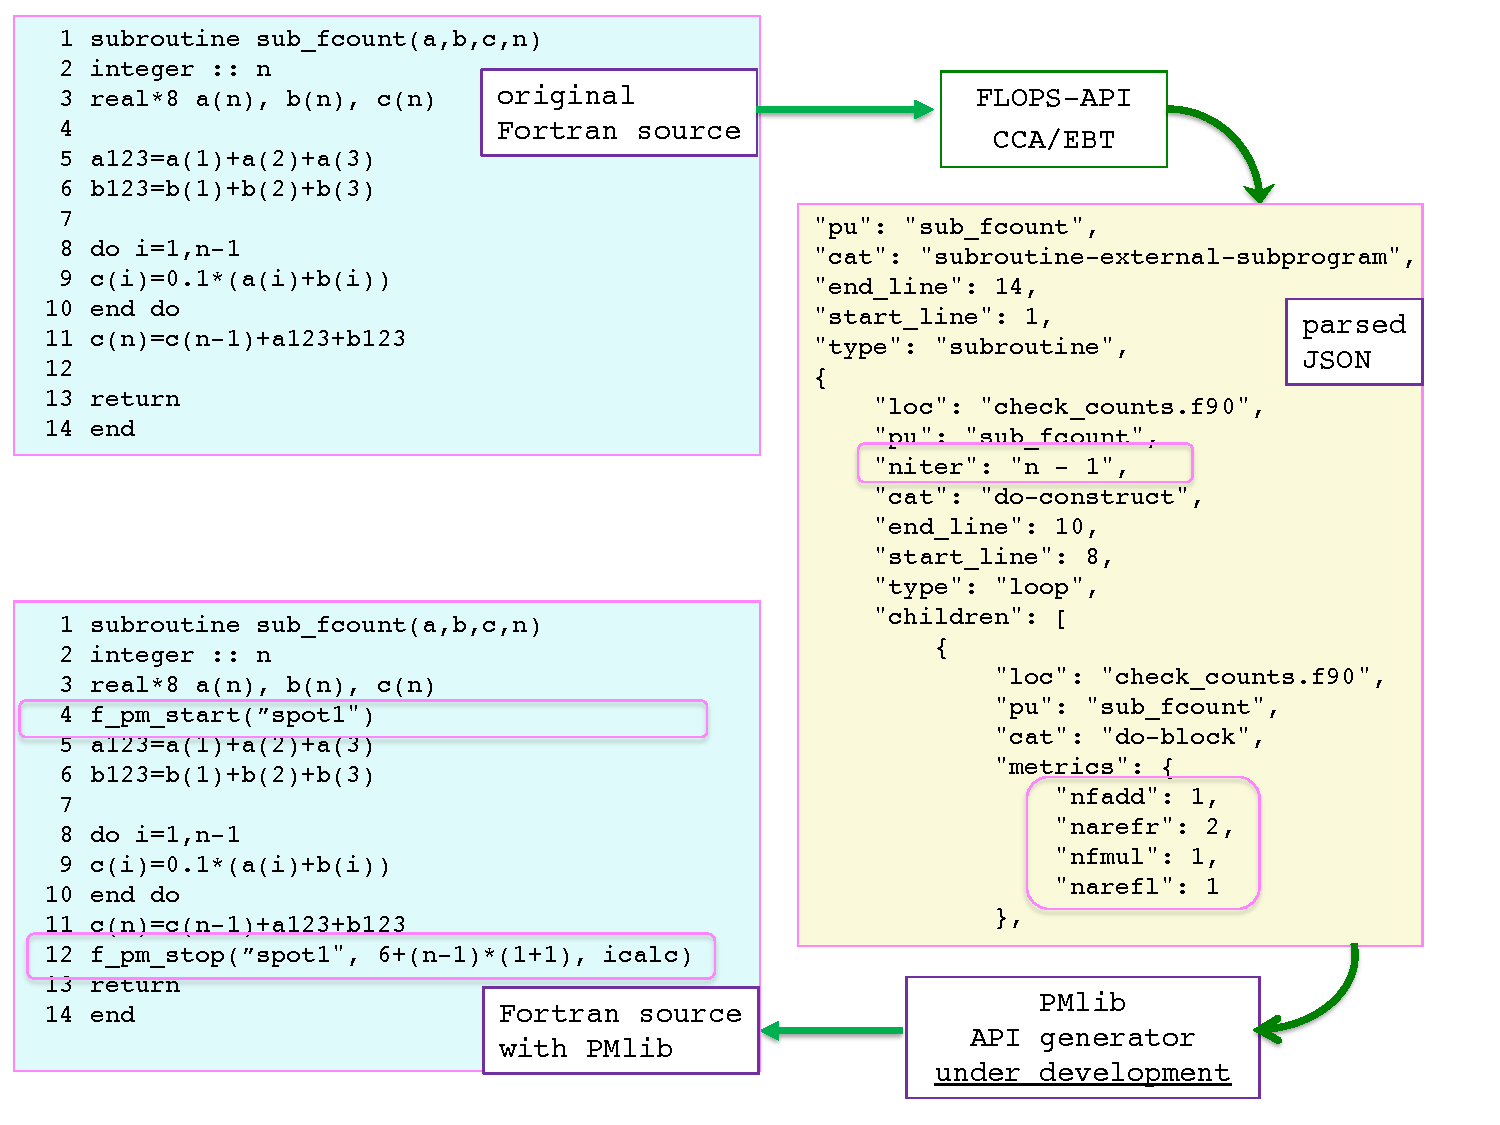
\includegraphics[width=0.5\textwidth]{figs/ccaebt4PMlib.pdf}
\caption{counting the operation with ccaebt}
\label{fig:ccaebt4PMlib}
\end{figure}

If HWPC workload is measured,
PMlib automatically detects the type of hardware, and reads the HWPC
event statistics at each of start/stop API.
In HWPC workload mode, PMlib does not use the user given argument value,
if any.
While PAPI has a good set of user APIs and is well documented,
it is not a simple task to choose the correct native event sets and masks
of the specific target processor instructions and to sort out the event
values for a desired performance category using a limited set of HWPC.
For example,
the standard output from papi\_native\_avail command on a server with
Intel Skylake Gold processor produces 5000+ lines.

PMlib takes the role to interface the application developer's intent to
categorize the raw performance information from HWPC, and to
help evaluate the performance.
Once PMlib APIs are coded in the application, PMlib preserves the HWPC
portability. That is, PMlib chooses and reads the appropriate HWPC event
set, if the application is run on different HPC systems.

\subsection{High resolution timer available to PMlib}
PMlib is a portable package, and utilizes linux standard timer
gettimeofday by default. It also has the installation option to utilize
a system specific high resolution low overhead timer if such timer is
available on the platform.

Fig.~\ref{fig:precise-timer} shows the comparison of standard timer and
high resolution timer on the two HPC systems in the previous section.
PMlib has provision to use them as installation option.

\begin{figure}[tb]
\centering
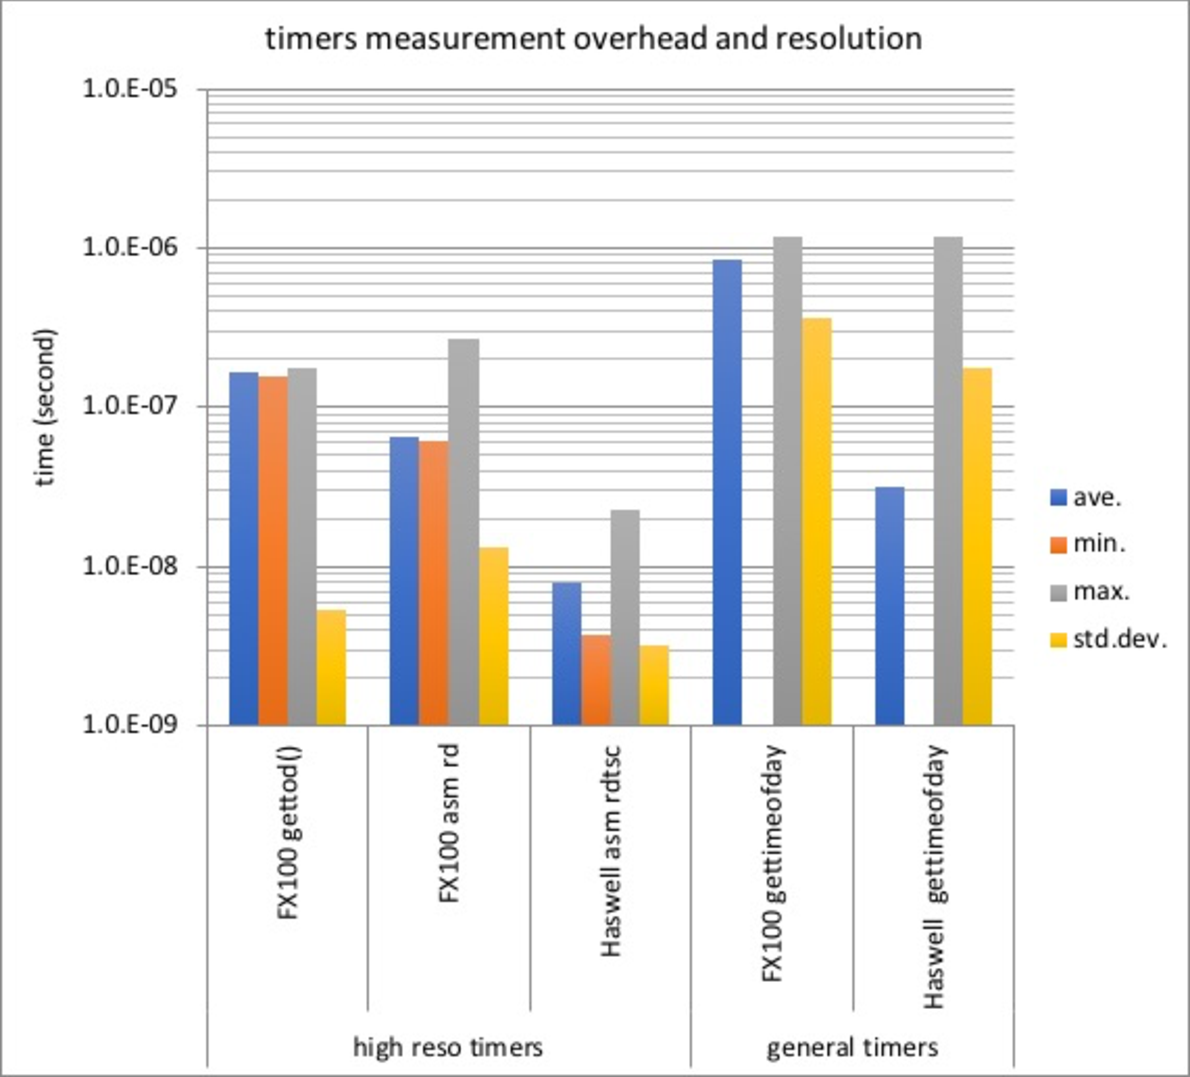
\includegraphics[width=0.45\textwidth]{figs/precise-timer.pdf}
\caption{comparison of accuracy between precise timer and general timer}
\label{fig:precise-timer}
\end{figure}

\subsection{Output information}
\label{subsection:PMlib-output-information}
The default output information from PMlib is a blocked text report based on
the time averaged performance statistics.
PMlib is also able to produce the Open Trace Format (OTF) tracing file
reflecting the shorter interval statistics for visualizatio.
%
%	OTF can be read by a Web browser visualization tool TRAiL.
%	\begin{figure}[tb]
%	\centering
%	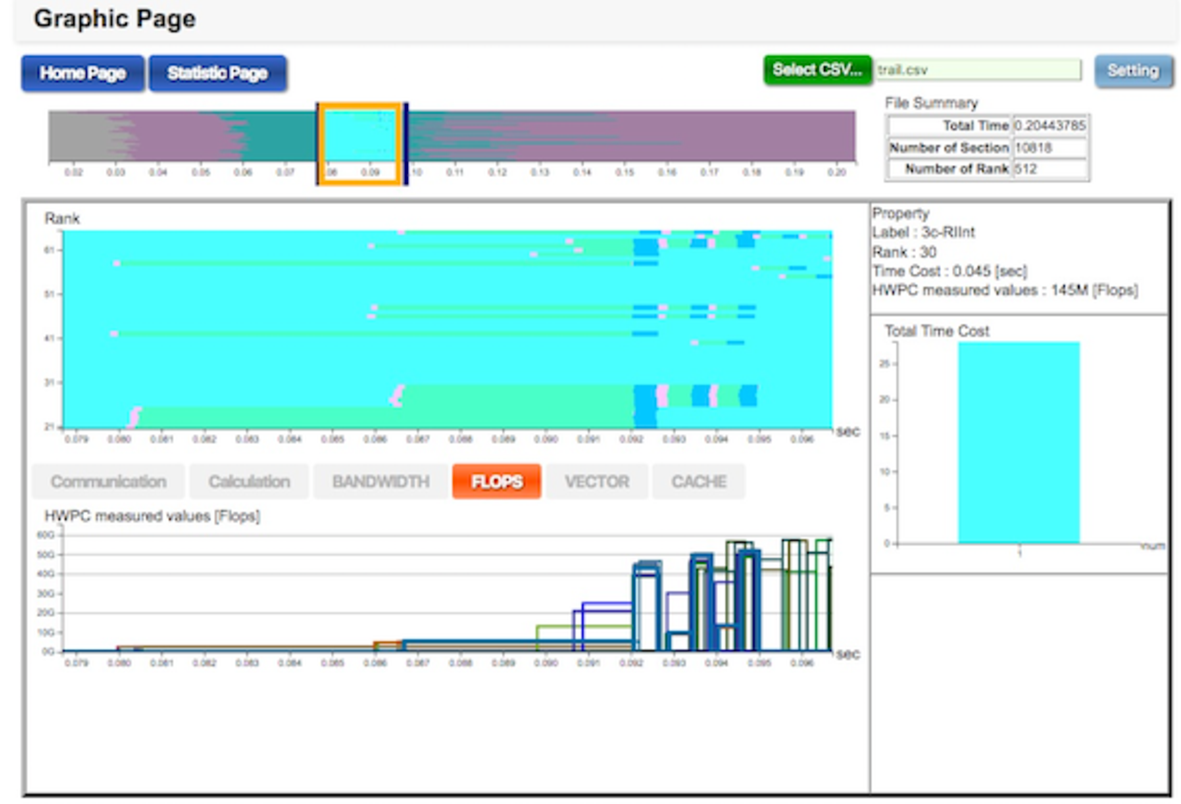
\includegraphics[width=0.45\textwidth]{figs/TRAiL-small.pdf}
%	\caption{tracing visualization using PMlib and TRAiL}
%	\label{fig:TRAiL}
%	\end{figure}

\subsection{other performance evaluation tools and related research}
\label{subsection:related-research}
There has been various tools developed for HPC system  performance evaluation.
Open source tools are designed to be portable.
Their functionalities are distinct, and in many cases multiple tools
are used in sequence to obtain the desired performance information.
These tools are classified as either sampling or tracing tool.
The overhead for using each tool is different.
Commercial vendor tools are used on many HPC systems.
They are best used for specific processor types.
HPC systems vendors also supply the performance evaluation tools
native to their systems.
They are integrated into systems and are easy to use in general,
but the availability is limited to the vendor's HPC systems only.

Some of the commonly used tools are listed below.
In the open source category:
\begin{itemize}
	\item Scalasca \cite{Scalasca:2017},\cite{Scalasca:2010}
			: trace generation, Score-P infrastructure
	\item Extrae \cite{Extrae:webpage} :  trace generation
	\item PAPI \cite{PAPI:5.6} : API to access HWPC
	\item Linux perf tools : API to access HWPC
\end{itemize}
In the commercial vendor category:
\begin{itemize}
		\item Intel VTune \cite{Intel:VTune} : Intel processors
		\item PGI Profiler \cite{PGI:Profiler} : X86 and GPU
\end{itemize}
These existing tools all utilize the processor performance information
based on HWPC workload, i.e. system workload.
PMlib appears to be the only tool that enables arithmetic and/or application
workload evaluation.

%%
\section{performance evaluation using PMlib}
\label{section:using-PMlib}

Some examples of using PMlib for performance evaluation are shown in this
section.
The list of servers used for the measurements are shown below.
\begin{itemize}
{
%	\setlength{\itemsep}{-5pt}
%	\setlength{\topsep}{2mm}
\item SGI Intel Ivybridge server
\item SGI Intel Skylake server
\item Fujitsu prime HPC FX100
}
\end{itemize}
The processor specifications and the major performance specifications
are listed in Table~\ref{tab:server-config}.

\newif\ifTwoservers
\newif\ifThreeservers
\Twoserversfalse
\Threeserverstrue
%\tiny
%\footnotesize
%\small
\begin{table}[tb]
\scriptsize
\caption{server configuration and hardware specification}
\label{tab:server-config}
\footnotesize

\ifTwoservers
\begin{tabular}{l|c|c} \hline
\scriptsize
system			&	FX100	&	Skylake	\\ \hline
CPU				&	SPARC64 XIfx	&	Gold 6148	\\ \hline
core GHz		&	1.975	&	2.4	\\ \hline
core Gflops	&	31.6	&	〜30	\\ \hline
L1\$ size (D,I)		&	64KB, 64KB	&	32KB, 32KB	\\ \hline
L1D\$ BW GB/s	&	140/R+70/W	&	154/R + 77/W	\\ \hline
\$ Linesize 	&	256B	&	64B	\\ \hline
L2\$ size		&	-	&	1MB	\\ \hline
L2\$ BW GB/s/core	&	-	&	154 ( ~70)	\\ \hline
LL\$ size		&	12MB	&	28MB(1.4MB/c)	\\ \hline
LL\$ BW GB/s/core	&	70/R+35/W	&	77 ( ~43)	\\ \hline
Memory			&	HMC(8x16Ls)	&	DDR4-2666	\\ \hline
Mem GB/s/[CMGcpu]	&	120/R+120/W	&	128	\\ \hline
\#cores/[CMGcpu]	&	16	&	20	\\ \hline
\end{tabular}
\fi

\ifThreeservers
\begin{tabular}{l|c|c|c} \hline
\scriptsize
Symbol			&	FX100	&	SKY		&	IVY \\ \hline
Platform		&	FX100	&	Skylake & Ivybridge\\ \hline
CPU				&	SPARC64 XIfx	&	Gold 6148	&	E5-4620v2	\\ \hline
core GHz		&	1.975	&	2.4	&	2.6 \\ \hline
core Gflops	&	31.6	&	~30	\\ \hline
\#core/cpu*	&	16	&	20	&	8	\\ \hline
L1\$ size(D,I)		&	64KB, 64KB	&	32KB, 32KB	\\ \hline
L1D\$ BW GB/s	&	140/R+70/W	&	154/R + 77/W	\\ \hline
\$ Linesize 	&	256B	&	64B	&	64B	\\ \hline
L2\$ size		&	-	&	1MB	&	256KB	\\ \hline
L2\$ BW GB/s/c	&	-	&	154 ( ~70)	\\ \hline
LL\$ size		&	12MB	&	28MB	&	20 MB	\\ \hline
LL\$ BW GB/s/c	&	70/R+35/W	&	77 ( ~43)	\\ \hline
Memory			&	HMC(8x16Ls)	&	DDR4-2666	& DDR3-1600	\\ \hline
Mem GB/s/cpu*	&	120/R+120/W	&	128	\\ \hline
\#cores/cpu*	&	16	&	20	\\ \hline
\multicolumn{4}{l}{\scriptsize\hspace{5mm} remark. cpu* indicates processor or
CMG }\\
\end{tabular}
\fi

\end{table}

%
\subsection{basic kernels}
\label{subsection:basic-kernels}

Basic kernels composed of four basic arithmetic operations and square root
are evaluated first.
Fortran source program for the measuring kernels is shown in List 1.

\begin{lstlisting}[caption={basic kernels}]
subroutine sub_add(a,b,c,n)
real a(n), b(n), c(n)  
do i=1,n
c(i)=a(i)+b(i)
end do
return
subroutine sub_fma(a,b,c,n)
real a(n), b(n), c(n)  
do i=1,n
c(i)=a(i)+b(i)*d
end do
return
subroutine sub_divide(a,b,c,n)
real a(n), b(n), c(n)  
do i=1,n
c(i)=b(i)/a(i)
end do
return
subroutine sub_sqrt(a,b,c,n)
real a(n), b(n), c(n)  
do i=1,n
c(i)=sqrt(a(i))
end do
return
\end{lstlisting}


These basic kernels are computed as single strided loops without dependencies,
and are expected to be efficiently processed taking advantage of parallel
execution pipelines and wide units.
In this paper, the term vectorization and SIMD are used synonymously.
%
% We must cut the following important remarks because of the short space.
%
\if 0
Computing time is measured for above subroutines many times.
After subtracting the calling overhead time,
the average computing time for each kernel is obtained.
Do loop cost is included in the average computing time.

Typical HPC systems are shared by many users and tend to suffer from
the perturbation influence called noise, caused by other processes,
shared file system, network with shared topology, etc.
more than on a small dedicated system.
It is not very easy even for this simple measurement to remove the noise
when measuring the small granularity computation time.
On user side, removing the noise can be addressed through statistic approach,
such as
adding additional outer loop for repeated measurement, and filter out
the measurements whose value is out of standard deviation.
\fi

Figure~\ref{fig:fx100-gflops-long-R8} shows the 
measurement of the basic kernels on FX100 system using the loop length of
\begin{math}
n=1,2,4,..,2^{26}
\end{math}
after removing the noise as above.

The displayed curves represent arithmetic performance.
The performance tends to improve according to the increase of
loop length until L1 cache size limit is reached, and drops to
the bandwidth constrained performance level of the next level cash.
This performance tendency matches the reports from other associated research.
In short loop region,
the overhead to process loop set-up and update can not be neglected,
the the performance is bound to data access latency.
In long loop region,
the the performance is bound to
L1\$ / L2\$ / LLC / memory bandwidth in the roofline \cite{Williams:2009}
envelop which is shown in Fig.~\ref{fig:roofline-fx100}

FX100 has SIMD 256bit wide arithmetic and data access instructions.
Its floating point operations can be sorted in width as below.
\begin{quote}
\begin{small}
\begin{verbatim}
fpdp1  : "1FLOPS_INSTRUCTIONS";
fpdp2  : "2FLOPS_INSTRUCTIONS";
fpdp4  : "4FLOPS_INSTRUCTIONS";
fpdp8  : "8FLOPS_INSTRUCTIONS";
fpdp16 : "16FLOPS_INSTRUCTIONS";
\end{verbatim}
\end{small}
\end{quote}
The floating point operation workload including single precision
and double precision data types is given as:
\begin{align}
	\mathrm{W}_{hwpc} & = \mathrm{fpdp1} + 2.0*\mathrm{fpdp2} + 4.0*\mathrm{fpdp4} \nonumber \\
			& + 8.0*\mathrm{fpdp8} + 16.0*\mathrm{fpdp1} 
\end{align}

\begin{figure}[tb]
\centering
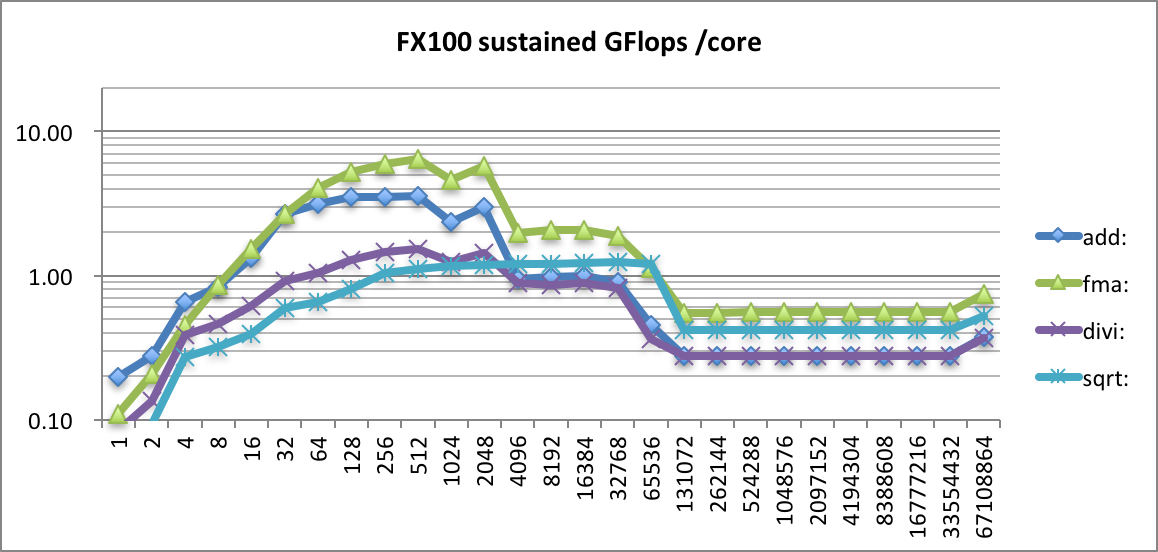
\includegraphics[width=0.45\textwidth]{figs/fx100-gflops-long-R8.pdf}
\caption{fx100-gflops-long-R8}
\label{fig:fx100-gflops-long-R8}
\end{figure}

\begin{figure}[tb]
%\begin{minipage}{0.48\hsize}
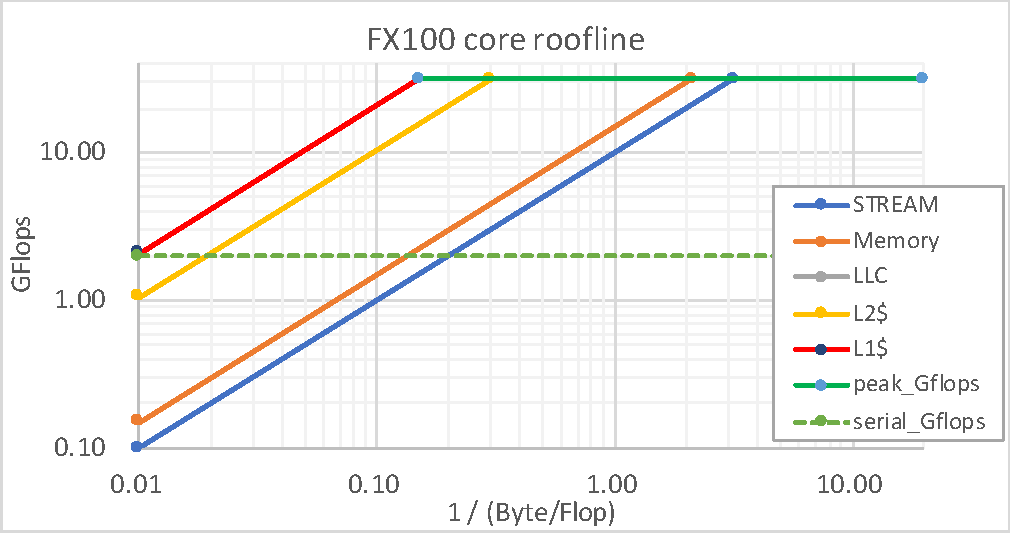
\includegraphics[width=0.45\textwidth]{figs/roofline-fx100.pdf}
\caption{roofline envelop FX100}
\label{fig:roofline-fx100}
\end{figure}
%\end{minipage}

PBlib HWPC report for some of above kernels is shown in
Table~\ref{tab:PMlib-report-HWPC}
Native HWPC events are sorted according to the choice of
environment variable HWPC\_CHOOSER explained in
\ref{subsection:Choosing-workload-type}
for user evaluation.
As read from the report,
the number of required operations for division is almost an order of magnitude
larger than addition, even though their arithmetic workload is same.
Division uses wider SIMD instruction, and has higher flop/byte ratio.
So division's apparent HWPC performanve becomes very high,
but the user perspective performamce is much lower than addition.
\begin{table*}[tb]
\scriptsize
\caption{PMlib HWPC report}
\label{tab:PMlib-report-HWPC}
\footnotesize
\input{figs/stdout.PMlib-report-HWPC.txt}
\end{table*}

%	
%
%	%\begin{minipage}{0.48\hsize}
%	%\end{minipage}
%
%	\begin{figure}[htb]
%	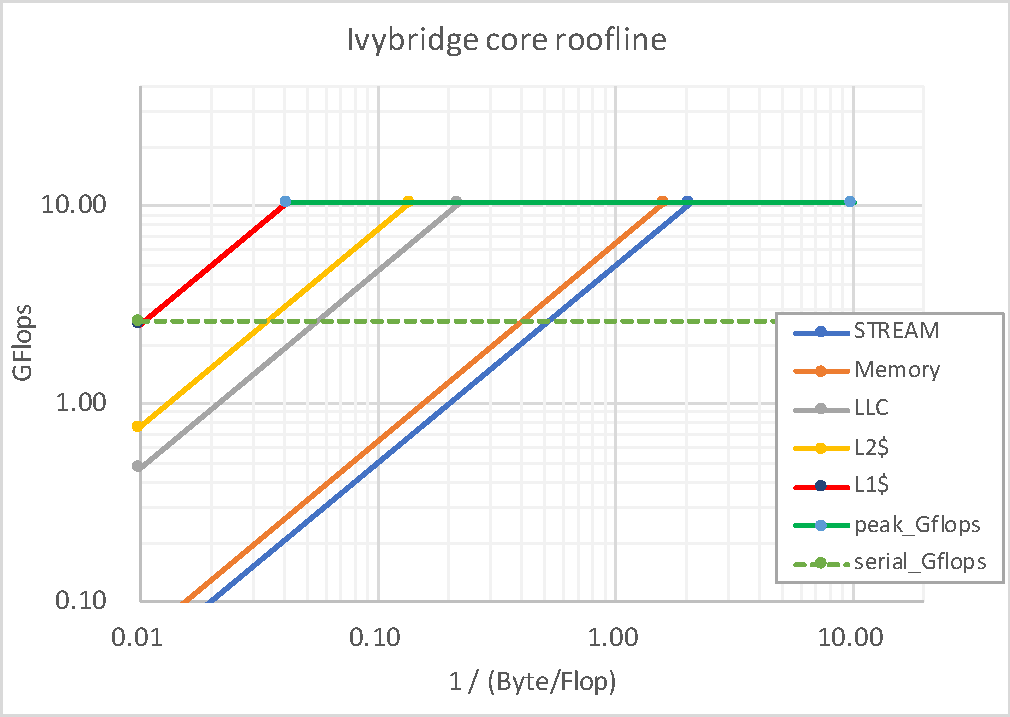
\includegraphics[width=0.45\textwidth]{figs/roofline-ivy.pdf}
%	\caption{roofline envelop IVY}
%	\label{fig:roofline-ivy}
%	\end{figure}


Figures~\ref{fig:fx100-gflops-short-R8}
shows the performance characteristics close-up of the same kernels for
\begin{math}
n=1,2,3,..,50
\end{math}
.
The close-up curves do not show gradual increase. Instead, they
show steep stepping shapes at multiple of constant interval.
This is a common observation on systems with SIMD supporting processors,
and the interval corresponds to the data width of SIMD instructions.
For example, FX100 double precision (64 bits) arithmetic can utilize
256 bit instruction, and the resulting interval is
\begin{math}
256 / 64 = 4
\end{math}
.
So the performance is highest at 4n, then 4n+1, 4n+2, and lowest at 4n+3.
Figure~\ref{fig:fx100-gflops-short-R8} is showing the fact that
program coding practice to maintain the loop length as the multiply of
SIMD width has significant impact, especially for short loop computation.
For single precision (32 bits), the interval becomes
\begin{math}
256 / 32 = 8
\end{math}
, and performance impact is even stronger as seen in
Fig.~\ref{fig:fx100-gflops-short-R4} for FX100.

\begin{figure}[tb]
\centering
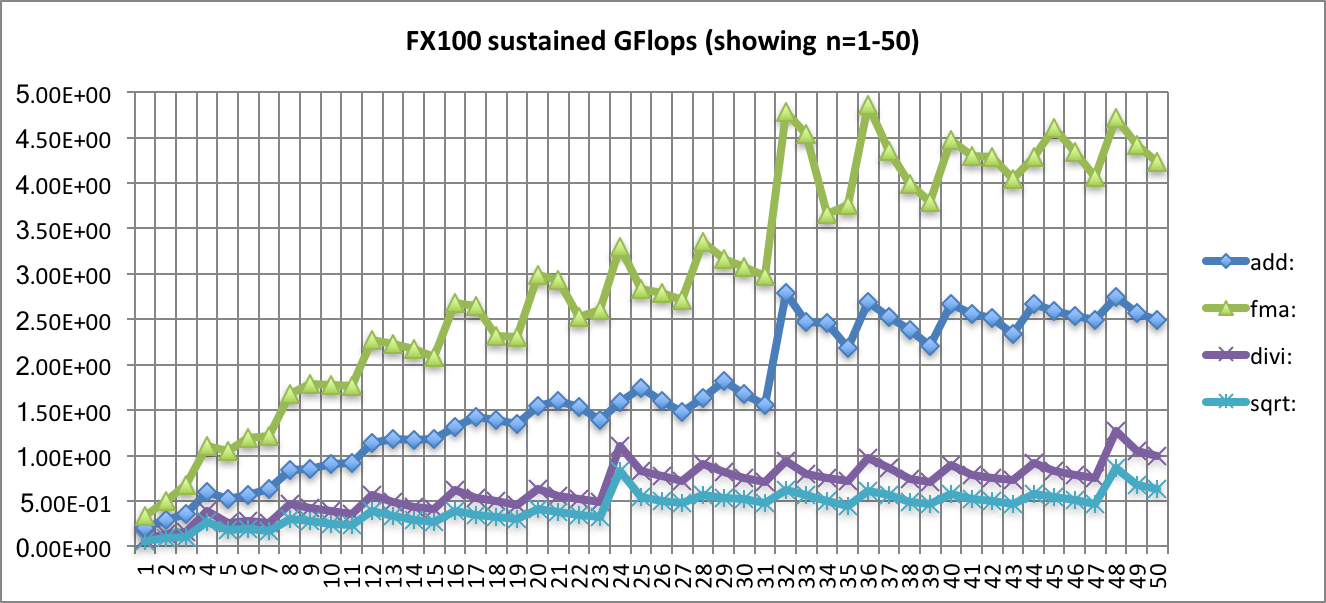
\includegraphics[width=0.45\textwidth]{figs/fx100-gflops-short-R8.pdf}
\caption{fx100-gflops-short-R8}
\label{fig:fx100-gflops-short-R8}
\end{figure}


\begin{figure}[tb]
\centering
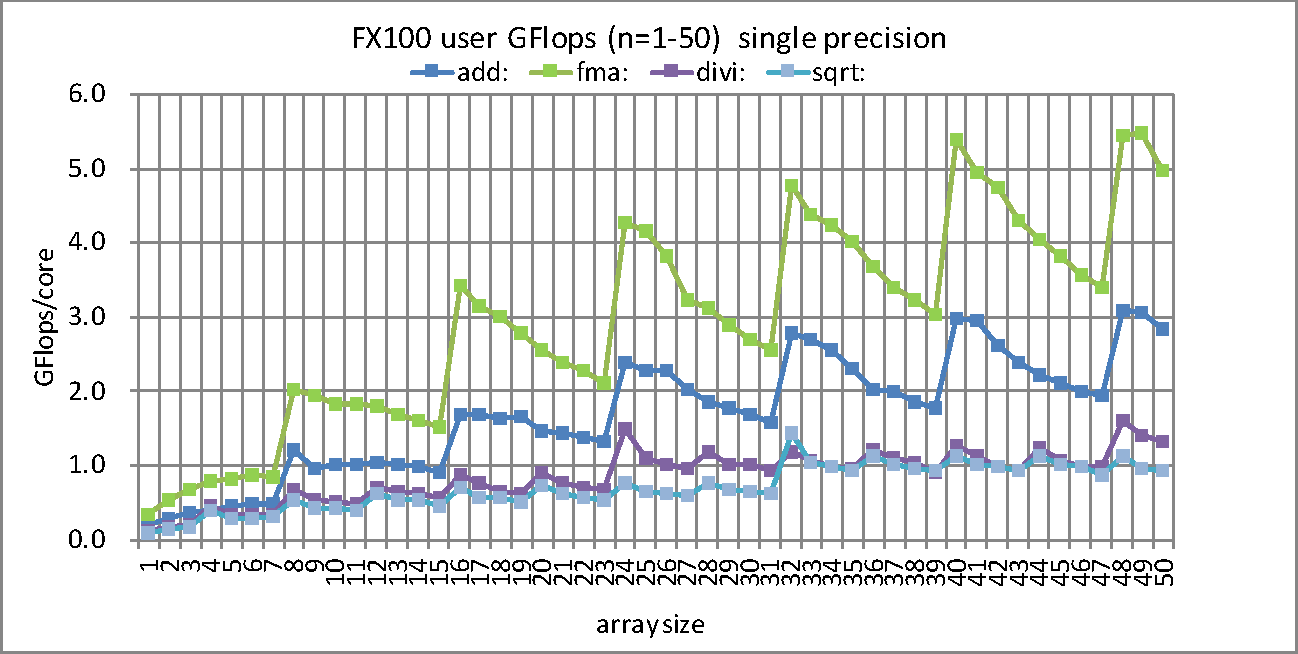
\includegraphics[width=0.45\textwidth]{figs/fx100-gflops-short-R4.pdf}
\caption{fx100-gflops-short-R4}
\label{fig:fx100-gflops-short-R4}
\end{figure}

Ivybridge also shows the similar curves.
Figure.~\ref{fig:ivy-gflops-short-R8} shows the double precision close up.
\begin{figure}[tb]
\centering
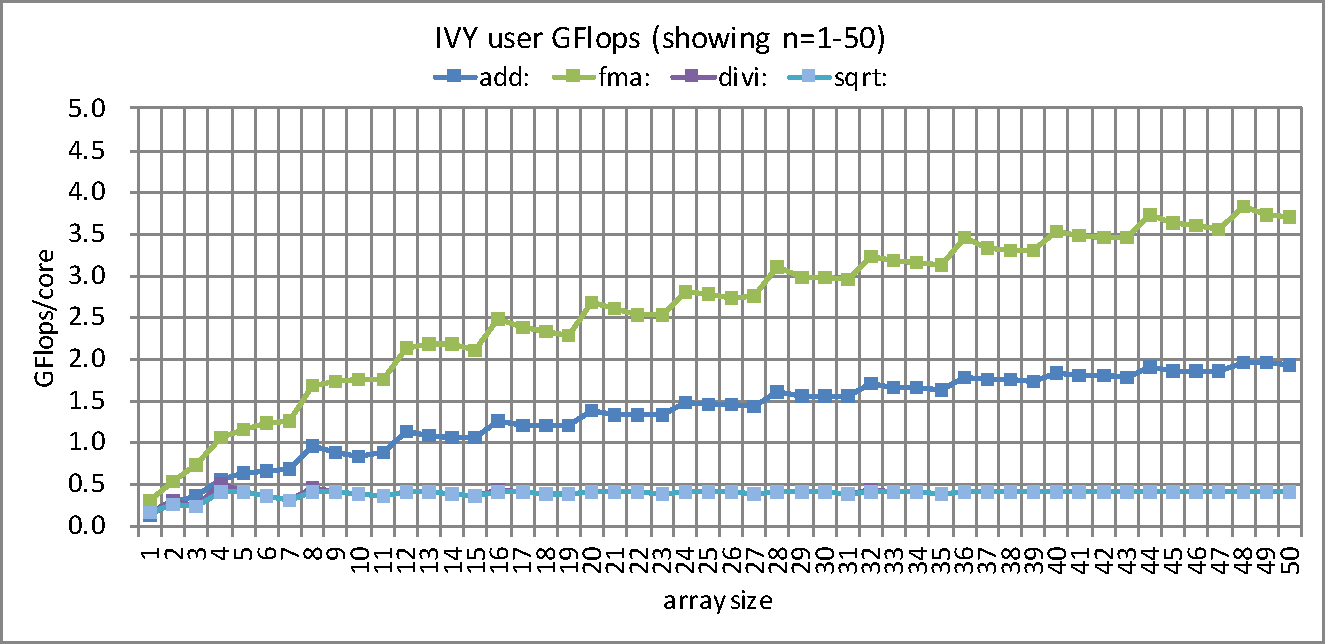
\includegraphics[width=0.45\textwidth]{figs/ivy-gflops-short-R8.pdf}
\caption{ivy-gflops-short-R8}
\label{fig:ivy-gflops-short-R8}
\end{figure}
Above example demonstrates the usefullness of conducting PMlib user mode
measurement and HPWC mode measurement in understanding the performance
gap within a program block of interest.

%
\subsection{STREAM}
\label{subsection:STREAM}
STREAM benchmark \cite{stream:1995}
has been widely used to measure the memory bandwidth of the computer systems.
STREAM standard output reports the
basic arithmetic performance of the copy, multiplication, addition,
and multiplication\&addition, i.e. arithmetic workload perspective.

STREAM HWPC performance shows different characteristics against
the reported STREAM arithmetic performance. Their performance is under
combined affect of compilers and their optimization options.
Although this paper does not intend to cover those exhaustive combinations,
a few points of interest related to the bandwidth are shown here.

The STREAM Fortran OpenMP result on IVY using 8 threads packed in a CPU
is shown first in fig.\ref{fig:stream-ivy-1cpux8T}.
Then we compare fig.\ref{fig:stream-ivy-1cpux8T}
with
fig.\ref{fig:stream-ivy-4cpux2T} 
which shows the result using 8 threads scattered over 4 CPUs.

The reported values by STREAM for packed thread assignment is better
if streaming-store option is used.
%
%	% minipage
%	\begin{figure}[tb]
%	\begin{minipage}{0.48\hsize}
%	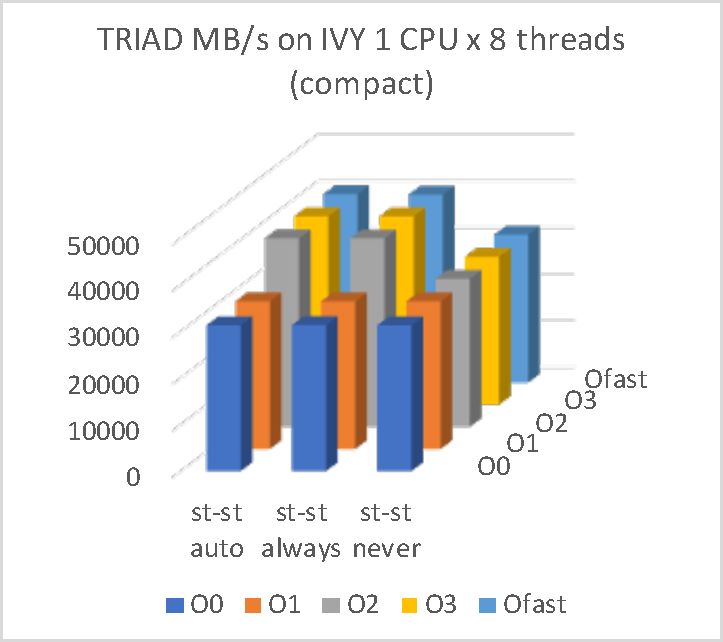
\includegraphics[width=0.98\textwidth]{figs/stream-ivy-1cpux8T.pdf}
%	\caption{stream-ivy-1cpux8T}
%	\label{fig:stream-ivy-1cpux8T}
%	\end{minipage}
%	\begin{minipage}{0.48\hsize}
%	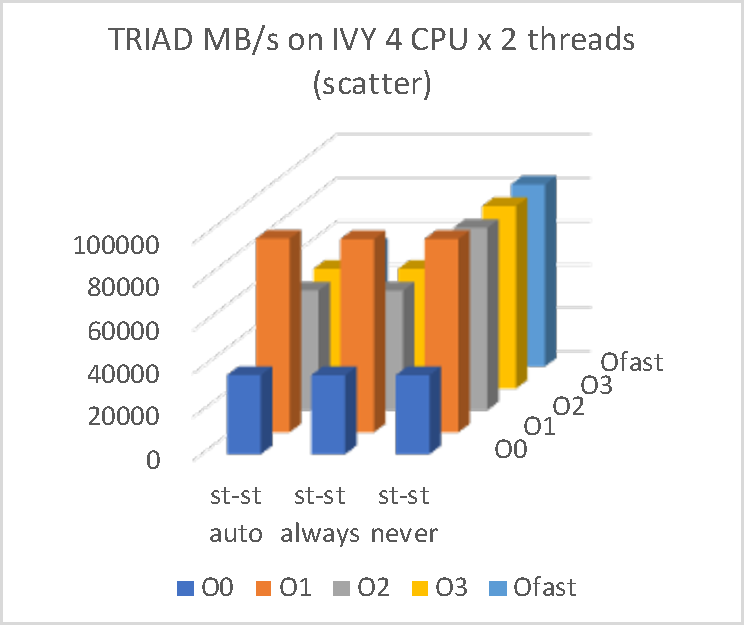
\includegraphics[width=0.98\textwidth]{figs/stream-ivy-4cpux2T.pdf}
%	\caption{stream-ivy-4cpux2T}
%	\label{fig:stream-ivy-4cpux2T}
%	\end{minipage}
%	\end{figure}
%
\begin{figure}[tb]
\centering
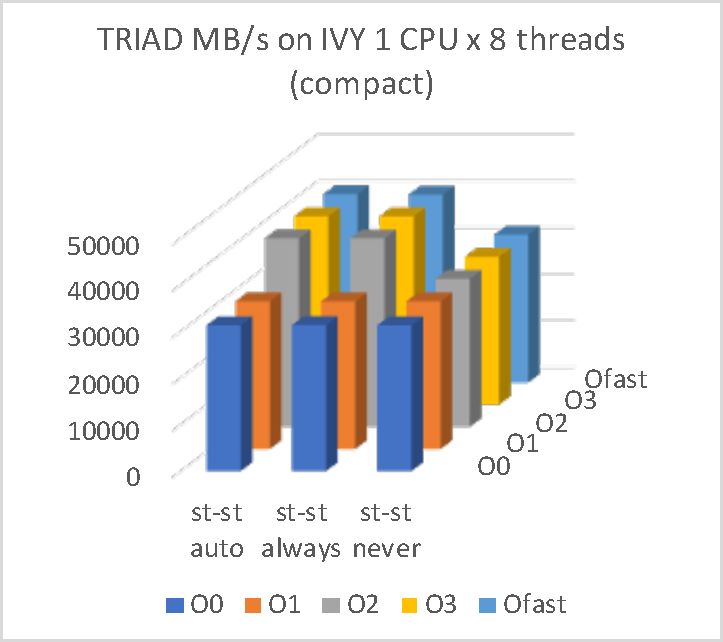
\includegraphics[width=0.45\textwidth]{figs/stream-ivy-1cpux8T.pdf}
\caption{stream-ivy-1cpux8T}
\label{fig:stream-ivy-1cpux8T}
\end{figure}
\begin{figure}[tb]
\centering
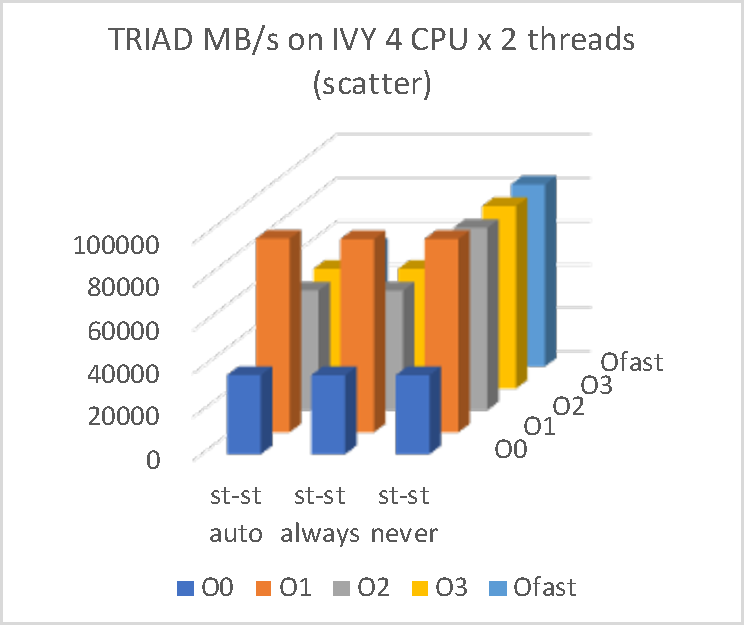
\includegraphics[width=0.45\textwidth]{figs/stream-ivy-4cpux2T.pdf}
\caption{stream-ivy-4cpux2T}
\label{fig:stream-ivy-4cpux2T}
\end{figure}
%
%%
\section{Conclusion}
In evaluating the applications performance on HPC systems, there can be
user perspective and system perspective, and they may exibit different
characteristis.
Evaluation from both perspectives provides the further understanding of
the performance model of the application on a specific HPC system.
PMlib provides the feature to conduct such synthetic performance
evaluation, and the hint for further optimized execution of
the application in its development and production phase.

\section*{Acknowledgment}
%	\section*{References}
\bibliographystyle{jplain}
\bibliography{PMlib}
\end{document}
